\documentclass[11  pt]{article} 
\usepackage[lmargin=1in,rmargin=1.75in,bmargin=1in,tmargin=1in]{geometry}  



% For hyperlinking everything
\usepackage{hyperref}
\hypersetup{
	colorlinks=true, %set true if you want colored links
	linktoc=all,     %set to all if you want both sections and subsections linked
	linkcolor=blue,  %choose some color if you want links to stand out
}


\usepackage[latin1]{inputenc}
\usepackage{amsmath}
\usepackage{mathrsfs}  
\usepackage{amsfonts}
\usepackage{amssymb}
\usepackage{graphicx}
\usepackage{subfig}
\usepackage{caption}
\usepackage{algorithm}
%\usepackage{algcompatible}
%\usepackage{algorithmicx}
\usepackage{algpseudocode}

\usepackage{titlesec}
\titleformat{\section}{\fontfamily{lmss}\fontsize{14}{15}\bfseries}{\thesection}{1em}{}
\titleformat{\subsection}{\fontfamily{lmss}\fontsize{12}{15}\bfseries}{\thesubsection}{1em}{}




\usepackage{amsthm}

\newtheoremstyle{noit}
{10pt}% <Space above>
{10pt}% <Space below>
{}% <Body font>
{}% <Indent amount>
{\bfseries}% <Theorem head font>
{.}% <Punctuation after theorem head>
{.5em}% <Space after theorem headi>
{}% <Theorem head spec (can be left empty, meaning `normal')>

\newtheoremstyle{example}
{10pt}% <Space above>
{10pt}% <Space below>
{}% <Body font>
{20pt}% <Indent amount>
{\bfseries}% <Theorem head font>
{.}% <Punctuation after theorem head>
{.5em}% <Space after theorem headi>
{}% <Theorem head spec (can be left empty, meaning `normal')>


\newtheoremstyle{indented}{20pt}{20pt}{\addtolength{\leftskip}{2.5em}}{}{\bfseries}{.}{.5em}{}


\newtheorem{theorem}{Theorem}
\numberwithin{theorem}{section}
\newtheorem{lemma}[theorem]{Lemma}
\newtheorem{corollary}[theorem]{Corollary}
\newtheorem{observation}{Observation}
%\numberwithin{observation}{section}
%\numberwithin{definition}{section}
\newtheorem{conjecture}{Conjecture}
\newtheorem{Qu}{Question}
\newcommand{\QU}{\begin{Qu}\normalfont}

\theoremstyle{noit}
\newtheorem{fact}{Fact}
\newtheorem{definition}{Definition}

\theoremstyle{indented}
\newtheorem{example}{Example}

\theoremstyle{indented}
\newtheorem{problem}{Problem}


%\newenvironment{proof}{\noindent{\bf Proof:} \hspace*{1em}}{
%    \hspace*{\fill} $\Box$ }
%\newenvironment{proof_of}[1]{\noindent {\bf Proof of #1:}
%    \hspace*{1em} }{\hspace*{\fill} $\Box$ }
%\newenvironment{proof_claim}{\begin{quotation} \noindent}{
%    \hspace*{\fill} $\diamond$ \end{quotation}}
\newcommand{\vs}[1]{\vspace{#1}}

\newcommand{\lecture}[2]{
 \noindent
\begin{center}
	\framebox{
		\vbox{
			\hbox to 5.78in { {\bf CSCE 411: Design and Analysis of Algorithms} \hfill  }
			\vspace{2mm}
			\hbox to 5.78in { {\Large \hfill Lecture #1\hfill} }
			\vspace{2mm}
			\hbox to 5.78in { {\it Date: #2 \hfill Lecturer: Nate Veldt} }
		}
	}
\end{center}
\vspace*{4mm}
}


\newcommand{\hw}[2]{
	\noindent
	\begin{center}
		\framebox{
			\vbox{
				\hbox to 5.78in { {\bf CSCE 411: Design and Analysis of Algorithms} \hfill  }
				\vspace{2mm}
				\hbox to 5.78in { {\Large \hfill Homework #1\hfill} }
				\vspace{2mm}
				\hbox to 5.78in { {\it Due date: #2 \hfil} }
			}
		}
	\end{center}
	\vspace*{4mm}
}



\newcommand{\under}[1]{\underline{\hspace{#1}}}
\setlength{\parindent}{0em}

%\usepackage[tagged]{accessibility}

% Graph terms
\newcommand{\vol}{\textbf{vol}}
\newcommand{\cut}{\textbf{cut}}


% Matrices
\newcommand{\mA}{\textbf{A}}
\newcommand{\mB}{\textbf{B}}

% vectors
\newcommand{\ve}{\textbf{e}}
\newcommand{\vx}{\textbf{x}}


% Other
\newcommand{\calN}{\mathcal{N}}

\usepackage{mathtools}
\DeclarePairedDelimiter\ceil{\lceil}{\rceil}
\DeclarePairedDelimiter\floor{\lfloor}{\rfloor}


\newcommand*{\aitem}{ \item[{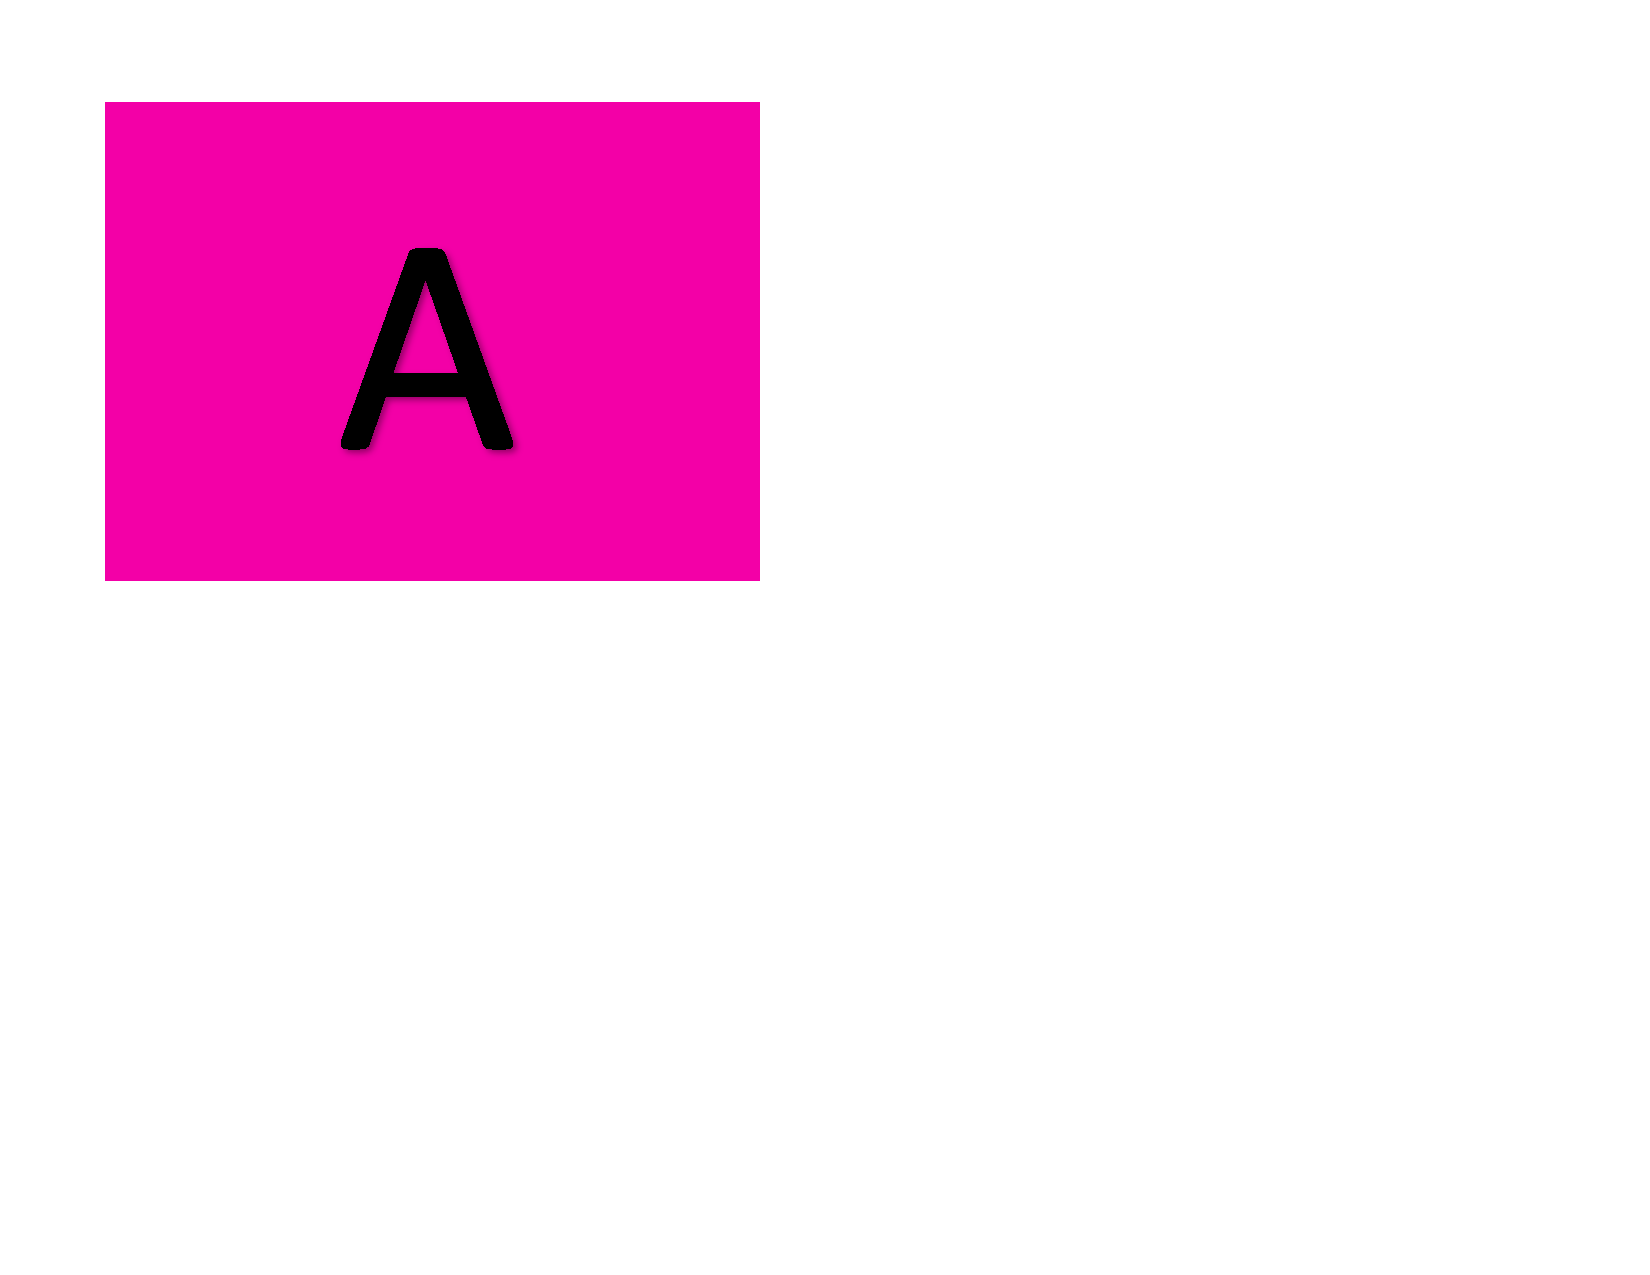
\includegraphics[width=0.8cm,height=0.5cm]{../../Lectures/figures/A}} ]  }
\newcommand*{\bitem}{ \item[{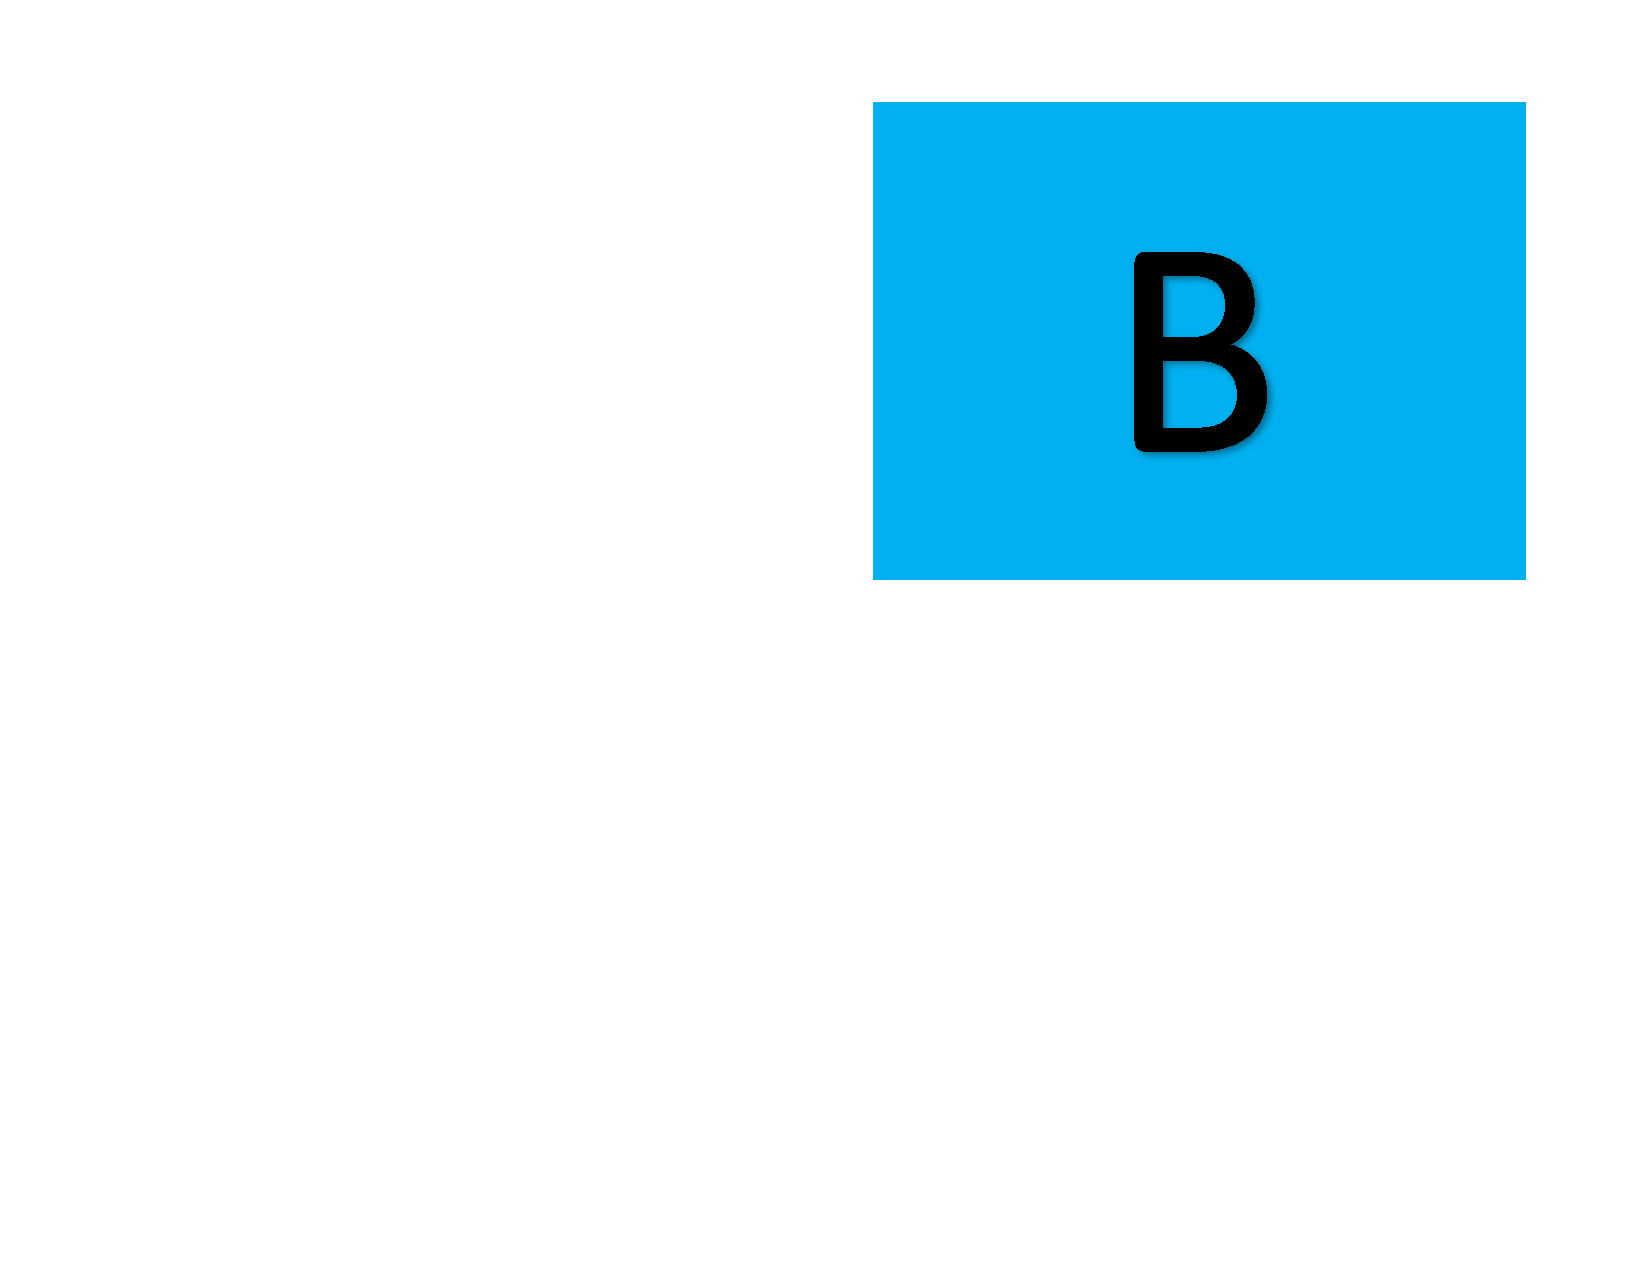
\includegraphics[width=0.8cm,height=0.5cm]{../../Lectures/figures/B}} ]  }
\newcommand*{\citem}{ \item[{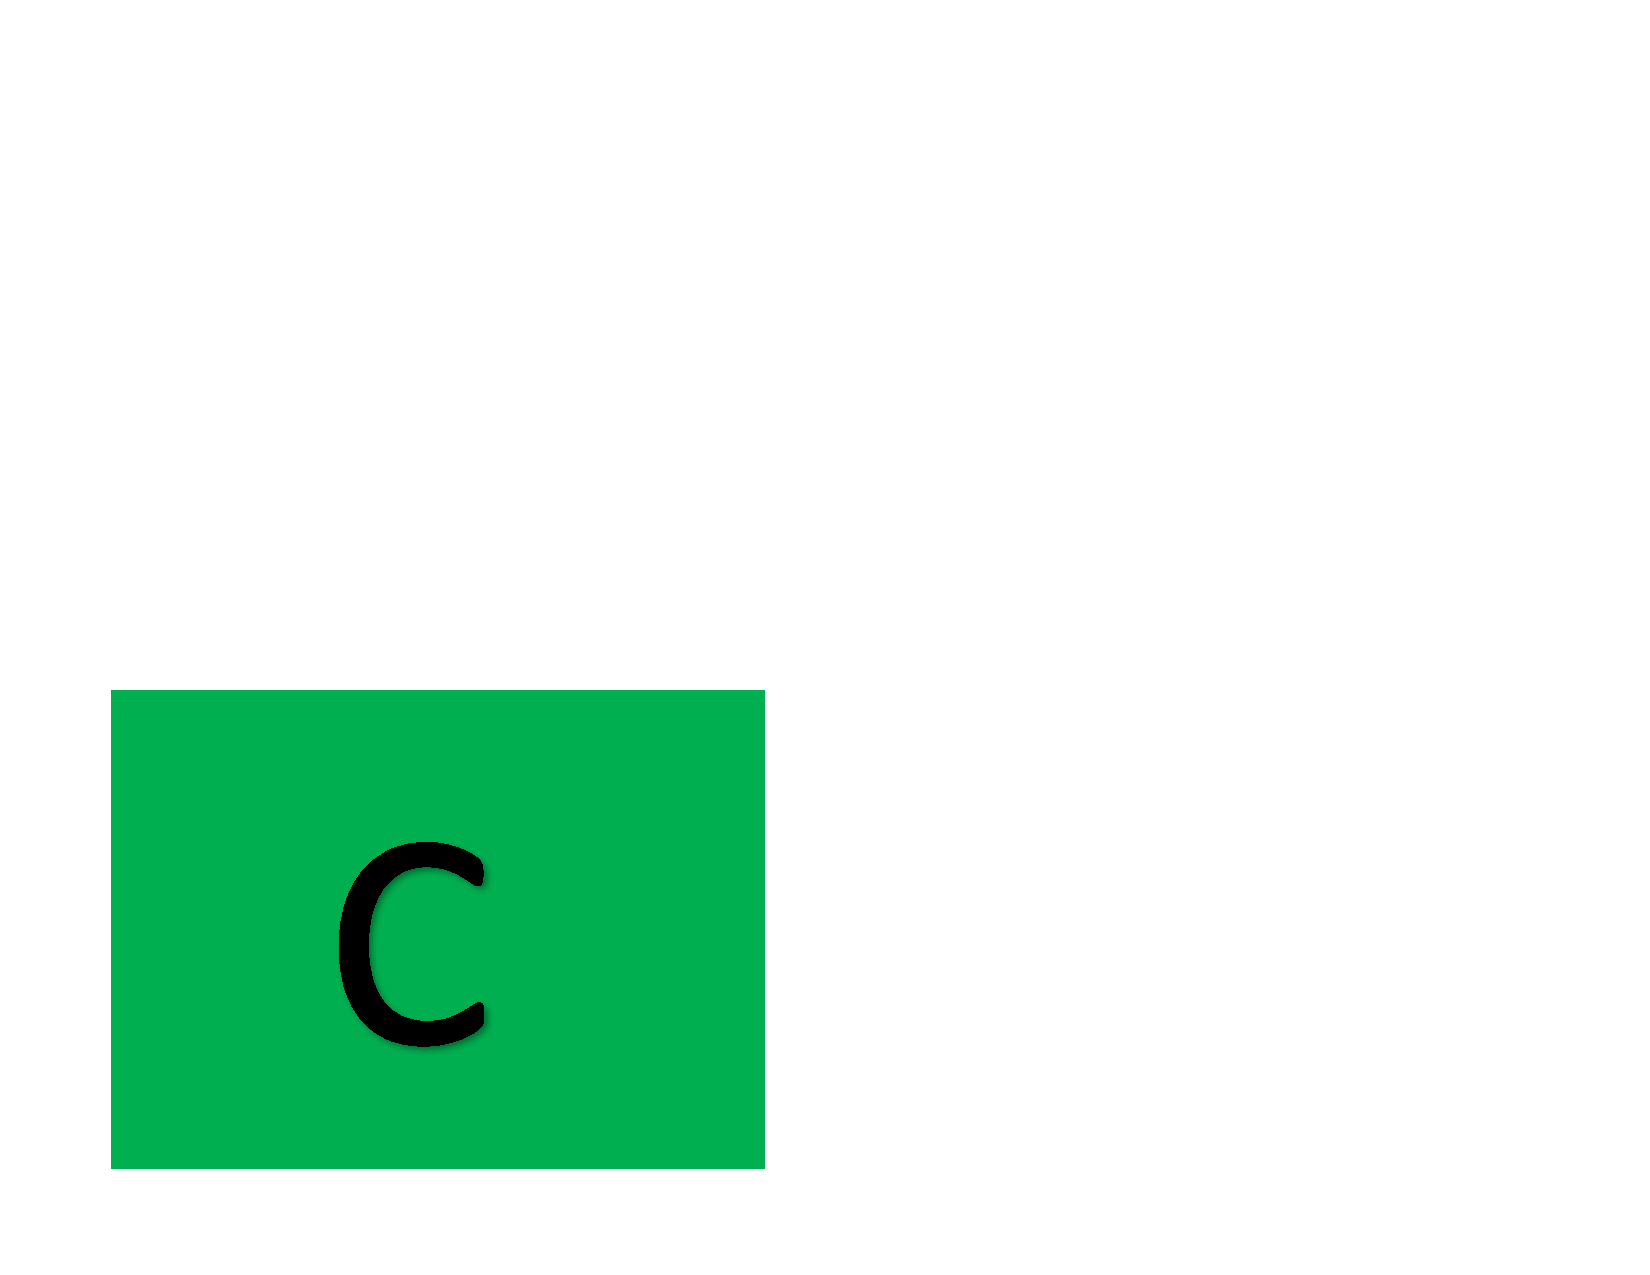
\includegraphics[width=0.8cm,height=0.5cm]{../../Lectures/figures/C}} ]  }
\newcommand*{\ditem}{ \item[{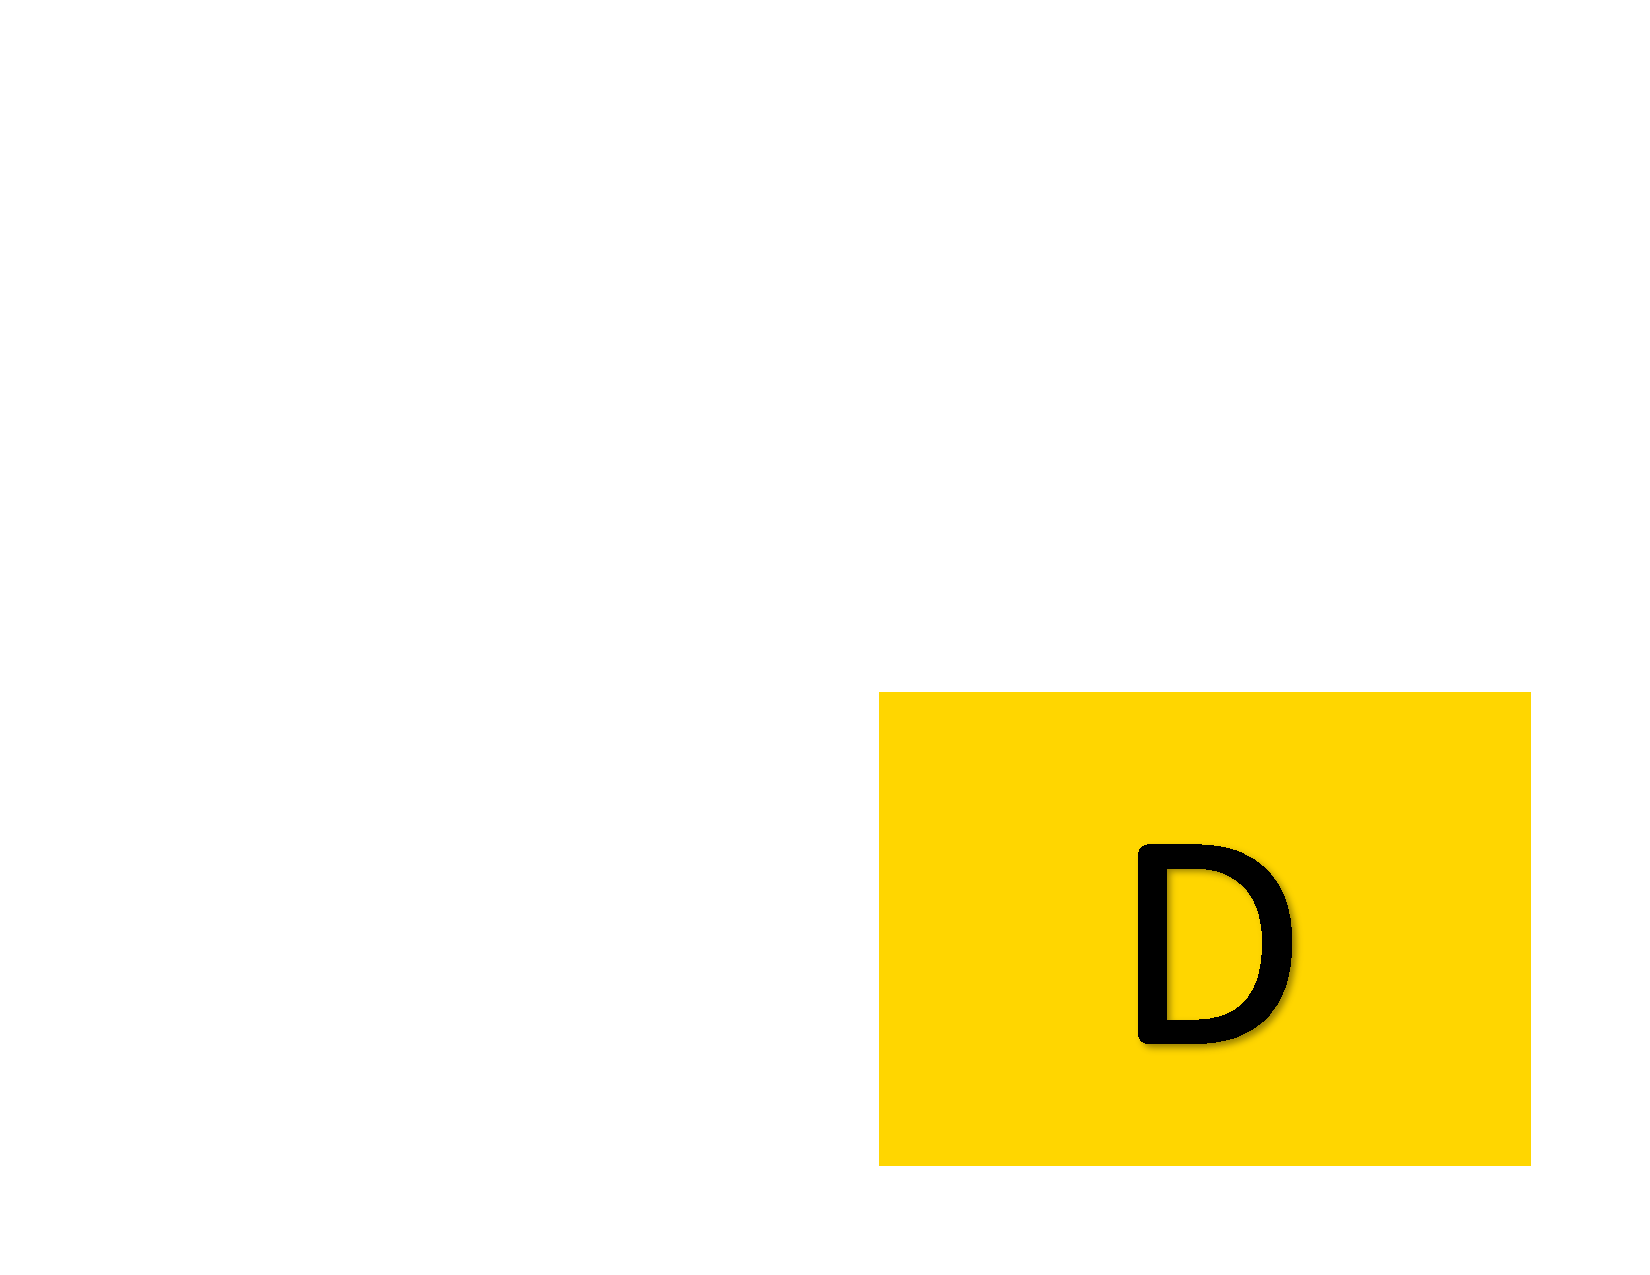
\includegraphics[width=0.8cm,height=0.5cm]{../../Lectures/figures/D}} ]  }
\newcommand*{\eitem}{ \item[{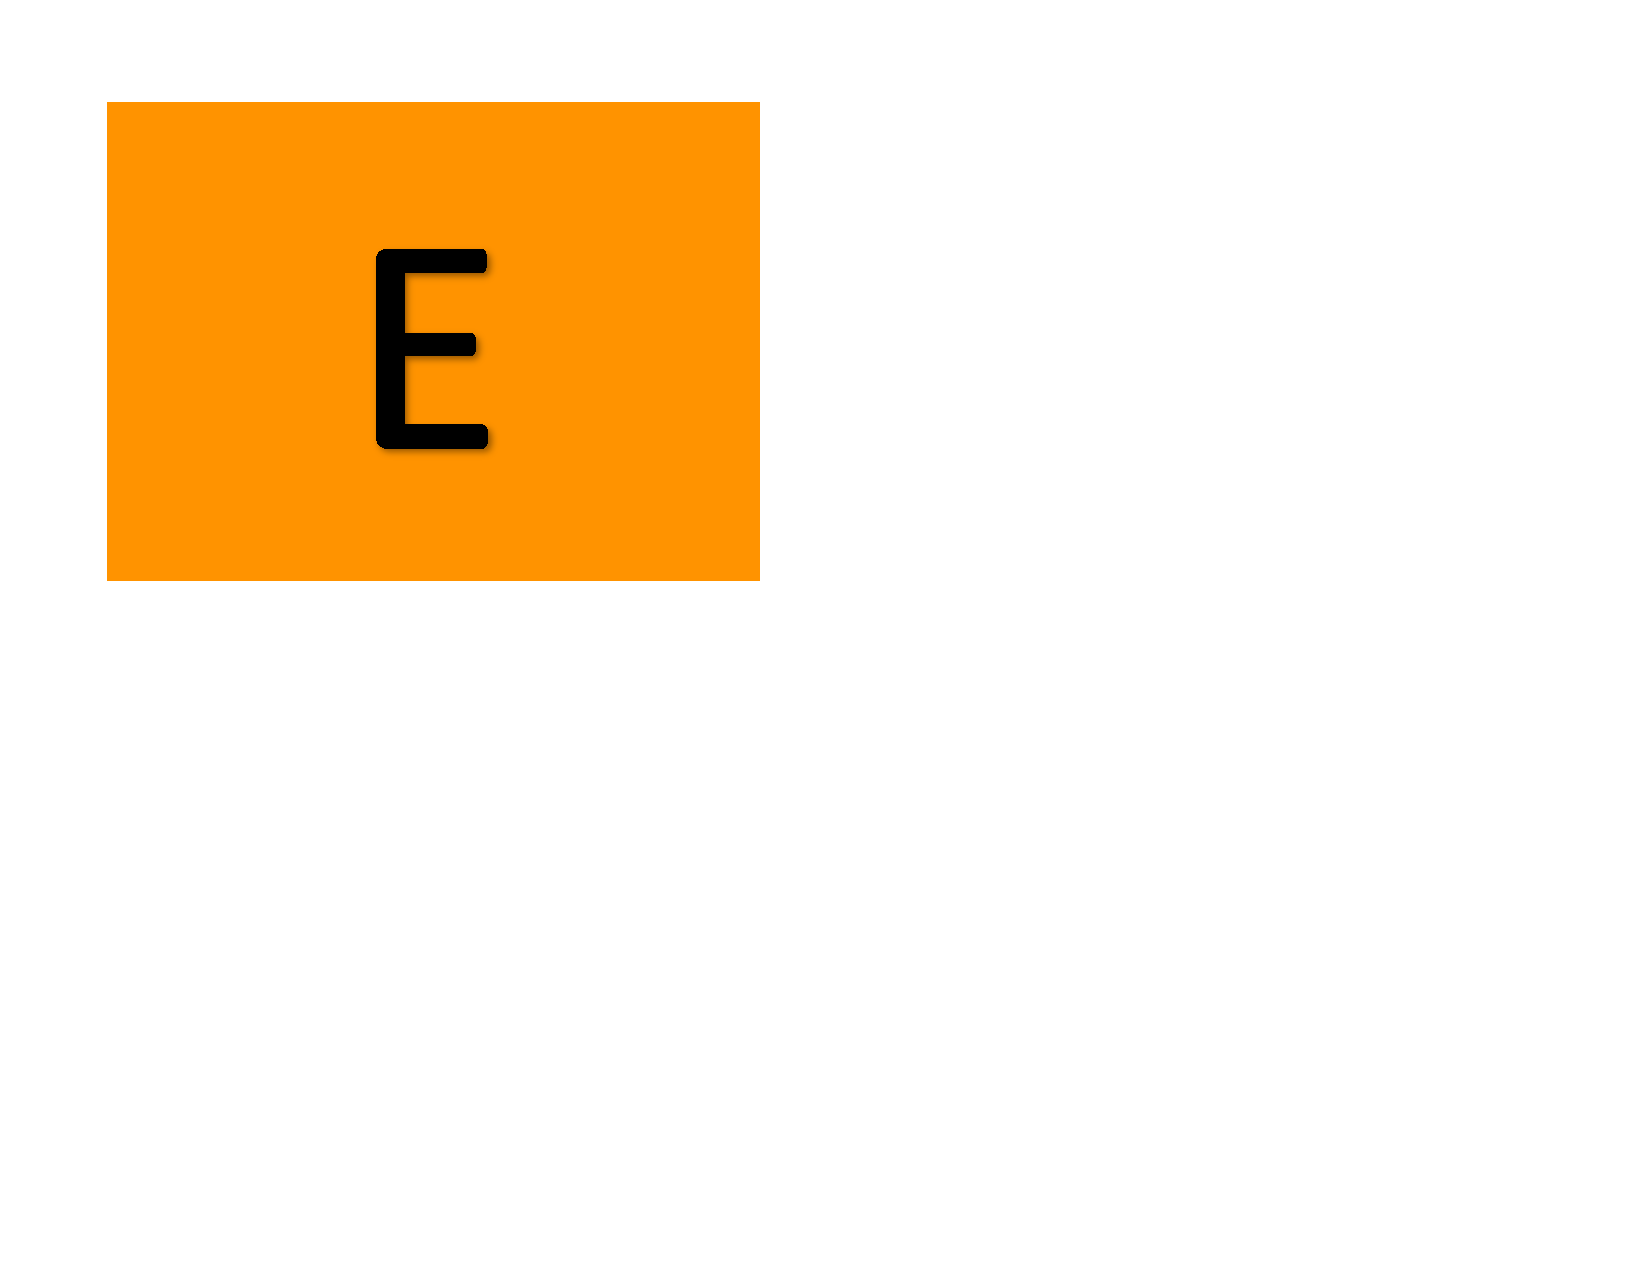
\includegraphics[width=0.8cm,height=0.5cm]{../../Lectures/figures/E}} ]  }
\newcommand*{\fitem}{ \item[{
\includegraphics[width=0.8cm,height=0.5cm]{../../Lectures/figures/F}} ]  }


\newcommand{\hide}[1]{\underline{\phantom{#1 #1}}}

\usepackage{setspace}

\onehalfspacing

\begin{document}


\lecture{0: Lecture Title}{Lecture date}

\section{Section}


\subsection{Subsection}

Some standard terminology for you to use:
\begin{itemize}
\item Undirected graph: $G = (V,E)$
\item  Use bold capital letters for matrices, like this $\mA$ or $\textbf{Q}$. 
\item Bold letters for vectors: $\vx$. 
\item Use the \verb|bmatrix| command for matrices.
\end{itemize}

\paragraph{Figures}
Figure~\ref{fig:1} is a triangle. When scribing, you do not need to figures for every picture drawn in class, but if you want to include figures, even if just simple ones, that's great! To do so, put all of your figures in a ``Figures'' file, and zip them up and send them along with the tex file and pdf. 
Call them in the text as follows

\begin{verbatim}
\begin{figure}[h!]
\centering
\includegraphics[width=0.25\textwidth]{Figures/triangle}
\caption{A figure}
\label{fig:1}
\end{figure}
\end{verbatim}


\begin{figure}[h!]
	\centering
	\includegraphics[width=0.25\textwidth]{triangle}
	\caption{A figure}
	\label{fig:1}
\end{figure}

\section{Some other general tips}

\begin{itemize}
	\item Always use math mode for mathematical objects, e.g. \verb|$V$| for node sets, and not just the letter V. 
	\item Don't put full words in math mode. If you have math and text mixed, use the \verb|\text{}| command. For example, to show ``$\vx \text{ and } \mA$'', use \verb|$\vx \text{ and } \mA$| and don't do \verb|$\vx and \mA$|. The latter looks bad: $\vx and \mA$.
	\item Pay close attention to spacing. If things look smashed together in math mode, in some cases it helps to add a space with the \verb|\,| command.
\end{itemize}

\section{Theorems, definitions, observations, etc.}

Professor Veldt will often label something as a ``definition'', ``theorem'', ``observation'', ``statement'', etc. In these cases, you the following environments (see .tex file).

\begin{definition}
	This is a definition. The sky is the blue thing above your head.
\end{definition}

\begin{observation}
	The sky is blue.
\end{observation}

\begin{fact}
	$L = \mB \mB^T$. (I'll use ``fact'' to denote a handy to know, that may require a proof in many cases, but is either too small or too informal a statement to be classified as a ``theorem'').
\end{fact}

\begin{theorem}
	This is a theorem. A big result that you will want to know. 
\end{theorem}

\begin{theorem}
	If I have another theorem in the same set of notes, the counter automatically gets updated so that this is Theorem 2.
\end{theorem}

\section{Submission}

If you are scribing for a lecture:
\begin{itemize}
	\item Scribe notes are due one week after lecture date.
	\item Simply email the .tex file, the .pdf file, and a zipped Figures folder (if you have any figures) directly to Professor Veldt.
\end{itemize}

\end{document}
